\section*{{Problem 2: Binäre Suchbäume}} 
\subparagraph*{a) Angenommen, wir haben einen binären Suchbaum T , welcher die Zahlen von
1 bis 1000 als Schlüssel speichert. Wir suchen in T nach dem Schlüssel 363.
Bestimmen Sie für jede der folgenden Schlüsselfolgen, ob sie als Folge der
Einträge auf dem Suchpfad nach 363 auftreten kann. Begründen Sie jeweils
Ihre Antwort.}


\begin{enumerate}
\item \textbf{2, 252, 401, 398, 330, 344, 397, 363.}

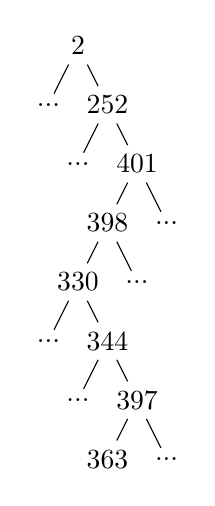
\begin{tikzpicture}[scale=0.5]

\node {2}
	child{node{...}}
	child{ node{252}
		child{node{...}}
		child{node {401}
			child{node{398}
				child{node{330}
					child{node{...}}
					child{node{344}
						child{node{...}}
						child{node{397}
							child{node{363}}
							child{node{...}}}}}
				child{node{...}}}
			child{node{...}}}};
\end{tikzpicture}

\begin{center}
\small
\hspace*{-1.5cm}
\begin{tabular}{@{} c c l c c @{}}
\toprule
\textbf{Schritt} & \textbf{Aktueller Knoten} & \textbf{Vergleich mit Ziel 363} & \textbf{Nächster Schritt} & \textbf{Intervall für nächsten Knoten} \\
\midrule
1 & 2   & \( 363 > 2 \Rightarrow \) rechts & 252 & \([3, 1000]\) \\
2 & 252 & \( 363 > 252 \Rightarrow \) rechts & 401 & \([253, 1000]\) \\
3 & 401 & \( 363 < 401 \Rightarrow \) links & 398 & \([253, 400]\) \\
4 & 398 & \( 363 < 398 \Rightarrow \) links & 330 & \([253, 397]\) \\
5 & 330 & \( 363 > 330 \Rightarrow \) rechts & 344 & \([331, 397]\) \\
6 & 344 & \( 363 > 344 \Rightarrow \) rechts & 397 & \([345, 397]\) \\
7 & 397 & \( 363 < 397 \Rightarrow \) links & 363 & \([345, 396]\) \\
8 & 363 & Ziel erreicht & — & — \\
\bottomrule
\end{tabular}
\end{center}


\item \textbf{924, 220, 911, 244, 898, 258, 362, 363.}

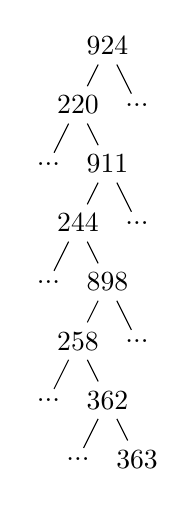
\begin{tikzpicture}[scale=0.5]
\node{924}
	child{node{220}
		child{node{...}}
		child{node{911}
			child{node{244}
				child{node{...}}
				child{node{898}
					child{node{258}
						child{node{...}}
						child{node{362}
							child{node{...}}
							child{node{363}}}}
					child{node{...}}}}
			child{node{...}}}}
	child{node{...}};
\end{tikzpicture}

\begin{center}
\small
\hspace*{-1.5cm}
\begin{tabular}{@{} c c l c c @{}}
\toprule
\textbf{Schritt} & \textbf{Aktueller Knoten} & \textbf{Vergleich mit Ziel 363} & \textbf{Nächster Schritt} & \textbf{Intervall für nächsten Knoten} \\
\midrule
1 & 924 & \( 363 < 924 \Rightarrow \) links & 220 & \([1, 923]\) \\
2 & 220 & \( 363 > 220 \Rightarrow \) rechts & 911 & \([221, 923]\) \\
3 & 911 & \( 363 < 911 \Rightarrow \) links & 244 & \([221, 910]\) \\
4 & 244 & \( 363 > 244 \Rightarrow \) rechts & 898 & \([245, 910]\) \\
5 & 898 & \( 363 < 898 \Rightarrow \) links & 258 & \([245, 897]\) \\
6 & 258 & \( 363 > 258 \Rightarrow \) rechts & 362 & \([259, 897]\) \\
7 & 362 & \( 363 > 362 \Rightarrow \) rechts & 363 & \([363, 897]\) \\
8 & 363 & Ziel erreicht & — & — \\
\bottomrule
\end{tabular}
\end{center}



\item \textbf{925, 202, 911, 240, 912, 245, 363.}

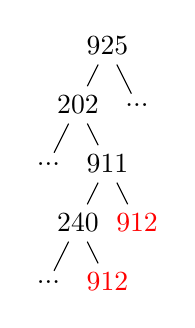
\begin{tikzpicture}[scale=0.5]
\node{925}
	child{node{202}
		child{node{...}}
		child{node{911}
			child{node{240}
				child{node{...}}
				child{node{\textcolor{red}{912}}}}
			child{node{\textcolor{red}{912}}}}}
	child{node{...}};
\end{tikzpicture}

\begin{center}
\small
\hspace*{-1.5cm}
\begin{tabular}{@{} c c l c c @{}}
\toprule
\textbf{Schritt} & \textbf{Aktueller Knoten} & \textbf{Vergleich mit Ziel 363} & \textbf{Nächster Schritt} & \textbf{Intervall für nächsten Knoten} \\
\midrule
1 & 925 & \( 363 < 925 \Rightarrow \) links & 202 & \([1, 924]\) \\
2 & 202 & \( 363 > 202 \Rightarrow \) rechts & 911 & \([203, 924]\) \\
3 & 911 & \( 363 < 911 \Rightarrow \) links & 240 & \([203, 910]\) \\
4 & 240 & \( 363 > 240 \Rightarrow \) rechts & 912 & \([241, 910]\) \\
5 & 912 & \( 363 < 912 \Rightarrow \) links & & \textcolor{red}{\( 912 > [910] \Rightarrow \) Fehler} \\
\bottomrule
\end{tabular}
\end{center}

\begin{itemize}
	\item Der Knoten 912 liegt nicht mehr im Intervall von [241,910] und somit ist der Knoten nicht in der \textbf{Schlüsselfolge}.
\end{itemize}

\item \textbf{2, 399, 387, 219, 266, 382, 381, 278, 363.}

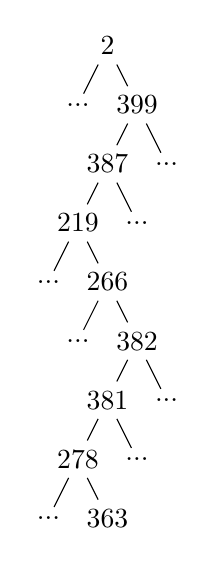
\begin{tikzpicture}[scale=0.5]
\node{2}
	child{node{...}}
	child{node{399}
		child{node{387}
			child{node{219}
				child{node{...}}
				child{node{266}
					child{node{...}}
					child{node{382}
						child{node{381}
							child{node{278}
								child{node{...}}
								child{node{363}}}
							child{node{...}}}
						child{node{...}}}}}
			child{node{...}}}
		child{node{...}}};
\end{tikzpicture}

\begin{center}
\small
\hspace*{-1.5cm}
\begin{tabular}{@{} c c l c c @{}}
\toprule
\textbf{Schritt} & \textbf{Aktueller Knoten} & \textbf{Vergleich mit Ziel 363} & \textbf{Nächster Schritt} & \textbf{Intervall für nächsten Knoten} \\
\midrule
1 & 2 & \( 363 > 2 \Rightarrow \) rechts & 399 & \([3, 1000]\) \\
2 & 399 & \( 363 < 399 \Rightarrow \) links & 387 & \([3, 398]\) \\
3 & 387 & \( 363 < 387 \Rightarrow \) links & 219 & \([3, 386]\) \\
4 & 219 & \( 363 > 219 \Rightarrow \) rechts & 266 & \([220, 386]\) \\
5 & 266 & \( 363 > 266 \Rightarrow \) rechts & 382 & \([267, 386]\) \\
6 & 382 & \( 363 < 382 \Rightarrow \) links & 381 & \([267, 381]\) \\
7 & 381 & \( 363 < 381 \Rightarrow \) links & 278 & \([267, 380]\) \\
8 & 278 & \( 363 > 278 \Rightarrow \) rechts & 363 & \([279, 380]\) \\
9 & 363 & Ziel Erreicht! & - & - \\
\bottomrule
\end{tabular}
\end{center}


\item \textbf{935, 278, 347, 621, 299, 392, 358, 363.}

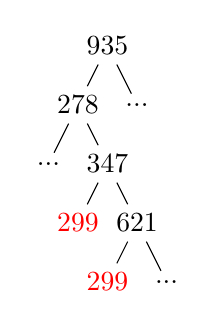
\begin{tikzpicture}[scale=0.5]
\node{935}
	child{node{278}
		child{node{...}}
		child{node{347}
			child{node{\textcolor{red}{299}}}
			child{node{621}
				child{node{\textcolor{red}{299}}}
				child{node{...}}}}}
	child{node{...}};
\end{tikzpicture}

\begin{center}
\small
\hspace*{-1.5cm}
\begin{tabular}{@{} c c l c c @{}}
\toprule
\textbf{Schritt} & \textbf{Aktueller Knoten} & \textbf{Vergleich mit Ziel 363} & \textbf{Nächster Schritt} & \textbf{Intervall für nächsten Knoten} \\
\midrule
1 & 935 & \( 363 < 935 \Rightarrow \) links & 278 & \([1, 934]\) \\
2 & 278 & \( 363 > 278 \Rightarrow \) rechts & 347 & \([279, 934]\) \\
3 & 347 & \( 363 > 347 \Rightarrow \) rechts & 621 & \([348, 934]\) \\
4 & 621 & \( 363 < 621 \Rightarrow \) links & 299 & \([348, 620]\) \\
5 & 299 & \( 363 > 299 \Rightarrow \) rechts & & \textcolor{red}{\( 299 < [348] \Rightarrow \) Fehler} \\
\bottomrule
\end{tabular}
\end{center}

\begin{itemize}
	\item Der Knoten 299 liegt nicht mehr im Intervall von [348,620] und somit ist der Knoten nicht in der \textbf{Schlüsselfolge}.
\end{itemize}


\end{enumerate}

\subsection*{b) Sei T ein binärer Baum mit n Knoten, und sei K eine total geordnete Menge
von n Schlüsseln. Zeigen Sie, dass es genau eine Möglichkeit gibt, die Schlüssel
aus K auf die Knoten von T zu verteilen, so dass die binäre Suchbaumeigen-
schaft erfüllt ist.} 

\textbf{Gegeben:}

\begin{itemize}
	\item $T$ ist ein binärer Baum mit $n$ Knoten
	\item $K = \{k_{1} < k_{2} < ... < k_{n}\}$ eine total geordnete Menge von $n$ Schlüsseln
	\item Dann gibt es genau eine Möglichkeit, die Schlüssel aus $K$ auf die Knoten von $T$ zu verteilen, sodass die binäre Suchbaumeigenschaft erfüllt ist.
\end{itemize}

\textbf{Induktionsanfang} \\
Ein Baum mit nur einen Knoten $n=1$ kann nur genau einen Schlüssel enthalten ( $K_{1}$ ), damit sind die BST(binary search tree)-Eigenschaften erfüllt.

\textbf{Induktionsvoraussetzung}\\
Wir nehmen an, dass das für alle binären Bäume mit weniger als $n$ Knoten zutrifft.

\textbf{Induktionsschritt} \\
$T$ ist nun ein binärer Baum mit $n \geq 2$ Knoten. \\
Dabei ist der linke Teilbaum $T_{L}$ und seine Knoten $n_{L}$, der rechte Teilbaum $T_{R}$ und seine Knoten $n_{R}$ \\
Es gilt: $n=n_{L} + 1 + n_{R}$ \\

Nun müssen wir die Schlüssel $K = \{k_{1} < k_{2} < ... < k_{n}\}$ auf die Knoten verteilen damit die BST-Eigenschaft noch erfüllt ist. \\

\begin{itemize}
	\item Dabei bekommt der Wuzelknoten von $T$ den Schlüssel $k_{n_{L}+1}$
	\item die kleineren Schlüssel landen in den linken Teilbaum $K_{L}$
	\begin{itemize}
		\item also kriegt der linke Teilbaum die $n_{L}$ Schlüssel $\{k_{1},...,k_{n_{L}}\}$
	\end{itemize}
	\item Schlüssel größer als der Wurzelknoten landen in dem rechten Teilbaum $T_{R}$
	\begin{itemize}
		\item also kriegt der rechte Teilbaum die $n_{R}$ Schlüssel $\{k_{n_{L}+2},...,k_{n}\}$
	\end{itemize}
\end{itemize}

$\Rightarrow$ Wenn wir das ganze nun auf die Induktionsvoraussetzung anwenden, erhalten wir für:
\begin{itemize}
	\item $T_{L}$ mit den Schlüsseln $n_{L}$ $\{k_{1},...,k_{n_{L}}\}$ $\Rightarrow$ genau eine Möglichkeit die Schlüssel zu verteilen, damit die BST-Eigenschaft gilt.
	\item $T_{R}$ mit den Schlüsseln $n_{R}$ $\{k_{n_{L}+2},...,k_{n}\}$ $\Rightarrow$ auch genau eine Möglichkeit die Schlüssel zu verteilen, damit die BST-Eigenschaft gilt.
	\item Damit das ganze funktioniert, muss die Wurzel genau den Schlüssel $k_{n_{L}+1}$ erhalten
\end{itemize}

Es gibt also für jeden binären Baum mit $n$ Knoten und jede total geordnete Menge von $n$ Schlüsseln genau eine Möglichkeit, die Schlüssel auf die Knoten zu verteilen, damit die BST-Eigenschaft erfüllt ist.
\begin{flushright}
$\Box$
\end{flushright}





 







